% PART I — FOUNDATIONS
\chapter{Chapter 1: Robotic Manipulation, Project Objectives, and Historical Scope}
\section{1.1 The Fundamental Challenge of Contact-Rich Manipulation}
Autonomous robotic manipulation differs profoundly from unconstrained motion planning or classical game benchmarks. When a 7-degree-of-freedom (7-DOF) serial manipulator approaches, grasps, lifts, transports, and inserts rigid objects in a tabletop workspace, control policies must negotiate discontinuous contact transitions, frictional shear limits across millimeter jaw apertures, non-convex kinematic joint bounds, partial observation noise, and severe long-horizon credit-assignment delays. A millimeter lateral misalignment or an excessive 0.14 m/s^2 vertical acceleration pulse at grasp closure can instantly break bilateral friction equilibrium and drop a payload.

The Dexterous-Robot-Learning project investigates how off-policy reinforcement learning (Soft Actor-Critic paired with Hindsight Experience Replay), dense potential shaping, progress-masked Behavioral Cloning, Hierarchical Reinforcement Learning (HRL), oblique RGB-D computer vision, and physics-informed inference shields can be systematically composed to achieve reliable simulated manipulation on the Franka Emika Panda platform under strict CPU-only single-process compute constraints.

\section{1.2 Verified Research Scope (Phases 1–17 Active; Phase 18 Proposed)}
Project development spans Phases 0 through 17 in verifiable simulation artifacts (PyBullet primary physics engine and MuJoCo 4.0.1 cross-simulator verification), alongside a refactored web-based simulation workstation built over FastAPI and Three.js. Phases 1–8 are reconstructed strictly from Git history (earliest commits 3a345f3, a5cc06b, 7ad9848 dated 2026-10-03), YAML snapshots, and TensorBoard scalars; where standalone historical artifacts (such as standalone Phase 5 notes) do not exist in the repository, they are explicitly documented as NOT RECOVERABLE FROM AVAILABLE EVIDENCE. Phase 17.3 hardware execution on physical Franka hardware was recorded as NOT\_ATTEMPTED, and Phase 18 (Multi-Agent Cooperative Manipulation) represents proposed future research scope only.

\begin{figure}[htbp]\centering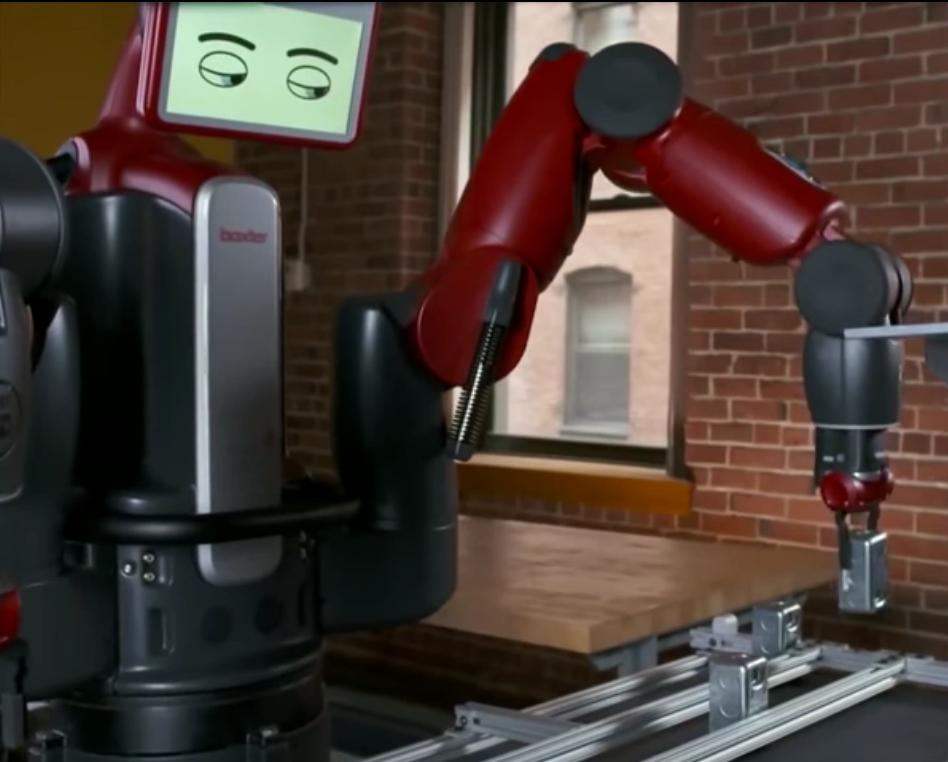
\includegraphics[width=0.9\linewidth]{../../assets/photographs/photo_03_research_lab_arm.jpg}\caption{Figure 1.1: Real-world laboratory compliant 7-DOF manipulator grasping a machined component above an industrial test rail. Source: Wikimedia Commons (File:Baxter\_1.jpg), Author: Salammbo31, License: CC BY-SA 4.0. Note: Illustrates general laboratory manipulation context; the current project evaluates Franka Panda strictly in simulation.}\end{figure}
\section{1.3 Franka Emika Panda Architecture and PyBullet Simulation Fundamentals}
In real industrial and university laboratories, torque-controlled 7-DOF collaborative manipulators such as the Franka Emika Panda provide kinematic redundancy: seven revolute axes allow reaching an arbitrary 6-DOF end-effector pose (position [x, y, z] and orientation [qx, qy, qz, qw]) while exploiting the extra null-space degree of freedom to avoid joint stops and singular elbow locking. Within simulation (`src/robots/panda.py`, wrapped cleanly in `robotics/robots/franka\_panda/robot\_model.py`), the official URDF `panda.urdf` models arm joints [0..6] with maximum effort limits [87, 87, 87, 87, 12, 12, 12] N*m, finger joints [9, 10] with 25 N maximum squeeze force over [0.00, 0.08] m aperture, and grasp target frame link 11 (`panda\_grasptarget`).

\begin{figure}[htbp]\centering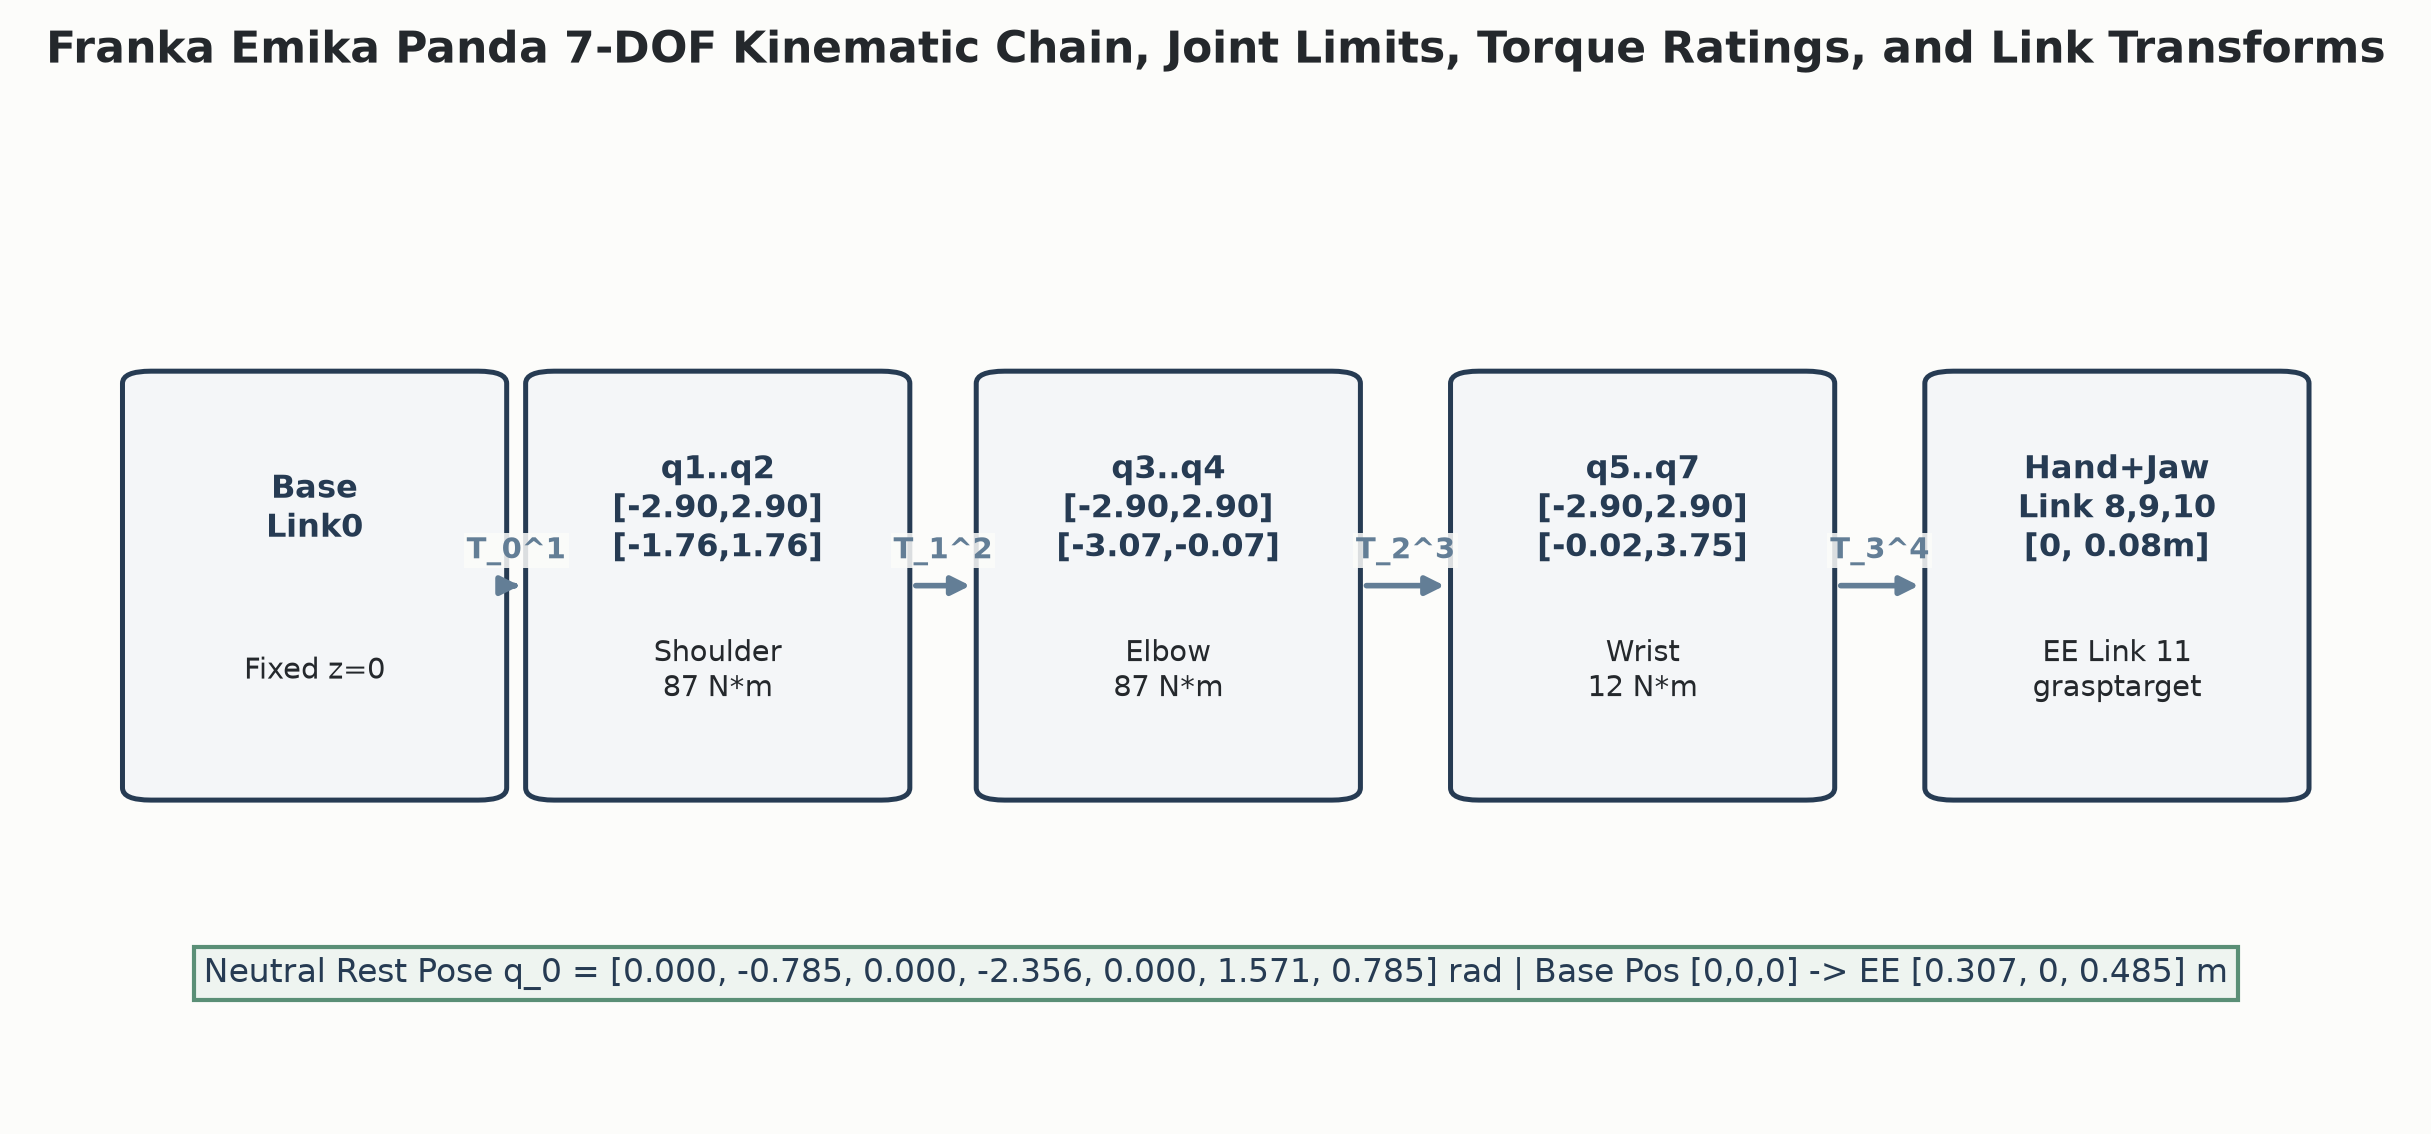
\includegraphics[width=0.9\linewidth]{../../assets/diagrams/diag_03_panda_kinematics_frames.png}\caption{Figure 1.2: Franka Emika Panda 7-DOF kinematic chain, effort ratings, joint limits, and neutral reference posture q\_0.}\end{figure}
\section{1.4 Real-World Applications and Engineering Relevance}
Manipulator architectures of this class underpin modern flexible automation across: (1) Industrial bin picking and machine tending (extracting randomized parts from shallow trays); (2) Warehouse order fulfillment and parcel sorting (rapid sequential color/SKU binning analogous to Phase 15.2 MultiSort); (3) Precision manufacturing assembly (connector mating and peg-in-slot insertion under lateral wall forces analogous to Phases 15.3 and 16.4); and (4) Healthcare and assistive robotics (adaptive object transfer near fragile surfaces). Deploying simulated policies onto hardware in any of these sectors would require empirical system identification, sensor calibration, real-time FCI driver certification (1 kHz control loop), and hardware safety interlocks beyond current simulation scope.
